\documentclass[12pt]{article}

\usepackage{enumerate}
\usepackage{rotating}
\usepackage{multicol}
\usepackage{multirow}
\usepackage{graphicx}
\usepackage{fullpage}
\usepackage{subfigure}
\usepackage{setspace}
\usepackage{listings}
\usepackage{lastpage}

\graphicspath{{./images/}}

% for references
\usepackage[pagebackref=false,colorlinks,linkcolor=blue,citecolor=magenta]{hyperref}
\usepackage[nottoc]{tocbibind}
\usepackage{fancyhdr}
\setlength{\headsep}{25pt}

\pagestyle{fancy}
\fancyhf{}
\lhead{\lr{Digital Image Processing}}
\rhead{تمرین اول}
\cfoot{صفحه \thepage\ از \pageref{LastPage}}
\lfoot{نیمسال مهر 00-99}
\rfoot{حمیدرضا ابوئی مهریزی}


% xepersian
\usepackage[extrafootnotefeatures]{xepersian}
\settextfont[Scale=1.4]{B Nazanin}
\setlatintextfont{Times New Roman}

\renewcommand{\labelitemi}{$\bullet$}

\begin{document}
	\doublespacing
	\begin{titlepage}
		\paragraph*{}
		\centering
			
			
			{\small به نام او}\\
			\vspace{1cm}
			\includegraphics[width=0.12\paperwidth]{aut.png}
			\hspace{1cm}
			\includegraphics[width=0.15\paperwidth]{DIP}
			\hspace{1cm}
			\includegraphics[width=0.12\paperwidth]{bme}\\
			\vspace{2cm}
			{\Huge پردازش تصویر}\\
			\vspace{2cm}
			{\large استاد : دکتر حامد آذرنوش}\\
			\vspace{0.5cm}
			{\small  دانشجو :‌ حمیدرضا ابوئی}\\
			\vspace{0.5cm}
			{\small شماره دانشجویی : 9733002}\\
			\vspace{0.5cm}
			{\small تمرین اول}\\
			\vfill
			{\tiny نیمسال مهر 00-99}
	\end{titlepage}
	\thispagestyle{plain}
	\tableofcontents
	\newpage
	%\onehalfspacing
	\doublespacing
	\section{سوال اول}
		\paragraph{توضیحات تکمیلی روند کد}
		بیشتر چیز ها واضح است، ‌در قسمت ج این سوال خواسته تا تعداد سطوح روشنایی را تغییر دهیم. من از تقسیم کردن، جزء صحیح گرفتن و سپس نرمال کردن به 0 تا 255 استفاده کردم و برای باینری کرددن نیز از 
		\lr{thresholding}
		  استفاده کردم.
		  
		اما در رابطه با اثر  تعداد سطوح روشنایی،این شکل با توجه به جزئیات زیاد شاید این تغییر تعداد سطوح در رتج های بالا زیاد مشهود نباشد اما اگر کمی دقیق شویم و یا تصویر دودویی را بررسی کنیم تفاوت با تصویر اصلی واضح است، در ضمن،این تغییر سطوح باعث میشود که ما در تغییرات سطوحی که زیاد تفاوت بین پیکسل ها نیست از هم گسستگی و شارپ بودن و مرز اشتباه حس کنیم
		
		در قسمت د، ابتدا میدانیم تصویر در اصل یک ماتریس است. برای نصف کردن تصویر، کافیست درایه هایی که نیاز داریم را در متغیر جدید بریزیم. برای نمایش نصف شدن نیز من دو تصویر نصف شده را پشت به پشت در کنار هم قرار دادم.
		
	برای وارون کردن نیز مطابق گفته‌ی بالا، باید ترتیب قرار گیری درایه ها را به نحوی قرار داد که درایه ها در آن محوری که مد نظر است، معکوس شوند 
	
		تغییر ابعاد روی رزولوشن عکس تاثیر مستقیم دارد زیرا ما تعداد داده ها را افزایش داده ایم بدون این که اطلاعاتمان بیشتر شده باشد. اما نکته اینجاست که ما با استفاده از درونیابی های مختلف میتوانیم تاثیر این موضوع را روی نتیجه ی خروچی کاهش دهیم و یک تصویر سافت تر یا هر درونیابی دیگری در خروجی به مخاطب نمایش دهیم.
		\paragraph{ورودی برنامه}
		
		
	 		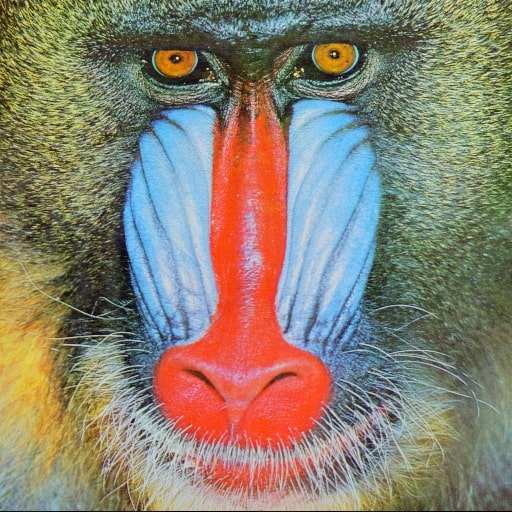
\includegraphics[scale=0.2]{inputs/mandrill.jpg}
		\paragraph{خروجی برنامه}.
		\lr{(512, 512, 3) <class 'numpy.uint8'> }
		
		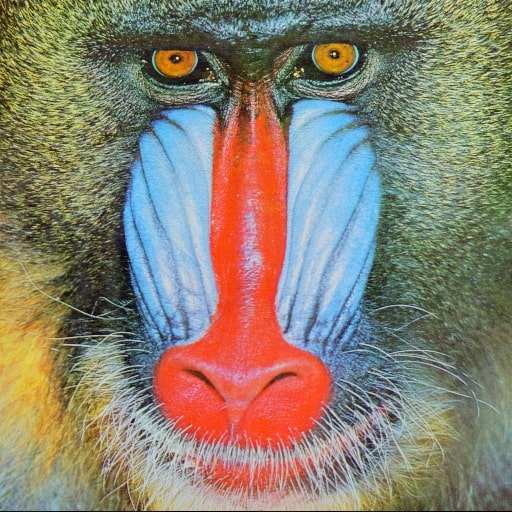
\includegraphics[scale=0.2]{one.png}
		\includegraphics[scale=0.2]{two.png}
 		\includegraphics[scale=0.2]{three.png}
 		\includegraphics[scale=0.2]{four.png}
 		\includegraphics[scale=0.2]{five.png}
 		\includegraphics[scale=0.2]{six.png}
 		\includegraphics[scale=0.2]{seven.png}
 		\includegraphics[scale=0.1]{eight.png}
 		\includegraphics[scale=0.1]{nine.png}
 		\includegraphics[scale=0.1]{ten.png}
 		\includegraphics[scale=0.2]{eleven.png}
  \newpage
  
  \section{سوال دوم}
  \paragraph{توضیحات تکمیلی روند کد}
ابتدا عکس را می‌خوانیم ‍‍سپس دو تثویر را در هم ضرب می‌کنیم.
برای این که دو تصویر را در هم ضرب کنیم دو روش وجود دارد. روش اول این است که دو تصویر را در هم ضرب کنیم و روش دوم آن است که تصویر دوم را به عنوان ماسک برای تصویر اول محسوب کرد. 
در قسمت ب
 ما تصویر را دریافت می‌کنیم و آن را به فضای 
 \lr{Gray scale}
 می‌بریم. حال در این فضا برای مکمل کردن، فضای کل یعنی 255 را از تصویر کم می‌کنیم. بنابراین جای سفید و سیاه عوض می‌شود و تصویر مکمل بدست می‌‌آید.
 حال برای تصویر اجتماع تصویر خاکستری و مکمل آن، چندین نظریه وجود دارد اولین نظریه این است که اگر ما شدت را در هر پیکسل برابر $x$ در نظر بگیریم اجتماع برابر می‌شود با 
 $uinon = (255 - x) + x = 255 $
 بنابراین تصویر نهایی ما برابر 255 خواهد بود که به معنی تصویر سفید است.
 
 در نظریه بعد به مفهوم مکمل و جبر مجموعه ها می‌پردازیم. 
 اگر ما مجموعه کل را $‌U$ بگیریم، تصویر خاکستری برابر $x$ و تصویر مکمل برابر $U-x$ خواهد بود، همانگونه که از تعریف مکمل بر می آید، هیچ اشتراکی با تصویر اصلی ندارد. بنابراین اجتماع این دو تصویر برابر خواهد بود با :
 $x \cup (U-x) = x + (U-x) -2* (x) \cap (U-x)$
 بنابراین برابر است با $U$ . 
 
 اختلاف دو تصویر را می‌توانیم با استفاده از تفریق کردن دو تصویر با استفاده از 
 $cv.subtract$
 به یک تصویر می‌رسیم و با نرمال کردن این تصویر به فضای 0 تا 255، تصویر ما به کنتراست خوبی می‌رسد. نتیجه رگ هایی است که در یک تصویر وجود دارد و در تصویر دوم وجود ندارد و تصویر دوم احتمالا با اضافه کردن ماده ی حاجب تولید شده است .
 


  \paragraph{ورودی برنامه}
  \includegraphics[scale=0.2]{inputs/x.jpg}
  \includegraphics[scale=0.2]{inputs/y.jpg}\\
  \includegraphics[scale=0.1]{inputs/a.jpg}
  \includegraphics[scale=0.1]{inputs/b.jpg}\\
  \includegraphics[scale=0.1]{inputs/c.jpg}
  \paragraph{خروجی برنامه}
  \includegraphics[scale=0.1]{one2.jpg}\\
  \includegraphics[scale=0.1]{two2.jpg}\\
  \includegraphics[scale=0.3]{three2.jpg}
  \includegraphics[scale=0.3]{four2.jpg}	

 	\newpage
	\section{سوال سوم}
	\paragraph{توضیحات تکمیلی روند کد}
	تبدیل خود را برای اعمال با تابع 
	\lr{wrapAffine}
	باید به شیوه ی 
	\begin{tabular}{ccc}
		
		\lr{Tx} & \lr{B} & \lr{A} \\
		\lr{Ty} & \lr{D} & \lr{C}\\
	\end{tabular}
بدهیم. اما اگر بخواهیم دستی ماتریس خود را اعمال کنیم کمی متفاوت است . در این مثال برای تغییر زاویه از روش دستی استفاده می کنیم و از دو روش مستقیم و معکوس بهره می‌بریم . راه مستقیم این است که تابع تبدیل خود را در مختصات ورودی ضرب کنیم و در خروجی مختصات تصویر را میگیریم و بدین صورت، تصویر نهایی درست می‌شود . در روش معکوس میاییم پیکسل های تصویر خروجی را در معکوس تابع تبدیل ضرب میکنیم تا مختصات ورودی ای که تحت آن تابع تبدیل به آن مختصات تصویر میشود را بیابیم. در روش مستقیم همانطور که در تصویر خروجی مشخص است برخی از نقاط که به نظر می‌رسد باید مقدار 255 داشته باشند، مقدار صفر دارند. این بدین معنی است که در این نقاط هیچ پیکسلی از تصویر ورودی تصویر نشده است. اما در روش معکوس که ‍ییکسل های خروجی مورد تحقیق قرار می‌گیرند، پیکسلی بدون مقدار باقی نمیماند اما در این روش نیز همچون روش قبل چون احتمال این که نقطه ی مرتبط با نقطه ی مورد بحث عدد صحیح نشود زیاد است، و در حقیقت ما با جزء صحیح گرفتن از مقدار به دست آمده یک تقریب میزنیم ، بنابراین در اطراف شکل برخی از نقاطی را مشاهده میکنیم که به علت همین تقریب ، مقدار نادرست نشان می‌دهند . که البته میتوان برای مثال با استفاده از روش های درونیابی مناسب این خطا را به حداقل رساند.

	   
	\paragraph{ورودی برنامه}
	پارامتر های ورودی به صورت زیر قرار داده شده است:
	\lr{Scaling: scale*1.5 \\ Translation : x:80 Pixel and y:-100 Pixel\\ Horizontal Sheer: 0.2 \\ Vertical Sheer: 0.2 \\ Rotation Forward: 0.5 rad \\Rotation Reverse: 0.3rad \\  }	
	
\includegraphics[scale=0.2]{inputs/T.jpg}\\

	\paragraph{خروجی برنامه}
	\includegraphics[scale=0.2]{images/one3.jpg}\\
	\includegraphics[scale=0.2]{images/two3.jpg}
	\includegraphics[scale=0.2]{images/three3.jpg}
	\includegraphics[scale=0.2]{images/four3.jpg}\\
	\includegraphics[scale=0.2]{images/five3.jpg}
	\includegraphics[scale=0.2]{images/six3.jpg}
	
	
	\newpage
	\raggedleft
	
\end{document}
